\documentclass[tikz,border=1pt]{standalone}
\usepackage{amsmath}
\usepackage{fontspec}
\setmainfont{Inter}[Scale=0.94]
\usetikzlibrary{positioning,arrows.meta,calc}
\definecolor{ink}{HTML}{0b0b0b}\definecolor{ink2}{HTML}{52514e}\definecolor{muted}{HTML}{8a8984}
\definecolor{rule}{HTML}{d9d8d2}\definecolor{paper}{HTML}{f6f5f1}
\definecolor{cblue}{HTML}{2a78d6}\definecolor{corange}{HTML}{eb6834}
% Designed at the ICLR text width (5.5 in = 139.7 mm), so it is included at 100% and text stays >= 6 pt.
\begin{document}
\begin{tikzpicture}[
  font=\fontsize{6.8}{8}\selectfont, ink,
  th/.style={inner sep=0pt, outer sep=0.3pt},
  lab/.style={font=\fontsize{6}{7}\selectfont, text=ink2},
  ttl/.style={font=\fontsize{7.2}{8.6}\selectfont\bfseries, anchor=base west},
  note/.style={font=\fontsize{6.2}{7.5}\selectfont, text=ink2, anchor=north west, align=left},
  box/.style={draw=rule, fill=paper, rounded corners=2pt, line width=0.5pt},
  stp/.style={draw=ink2, rounded corners=2pt, line width=0.5pt, fill=white, align=center,
              minimum height=10mm, text width=20.8mm, inner sep=1pt, font=\fontsize{6.1}{7.3}\selectfont, anchor=west},
  arr/.style={-{Stealth[length=1.3mm,width=1.1mm]}, line width=0.55pt, ink2},
  leak/.style={corange, line width=0.85pt, -{Stealth[length=1.3mm,width=1.1mm]}},
]
\def\w{7mm}\def\g{7.9mm}
% ================= (a) =================
\node[ttl] at (0, 33mm) {(a) A pre-augmented release};
\foreach \name [count=\v from 0] in {Original,Flip,Rotate,CLAHE,Gray,Black-hat}
  \node[lab, anchor=base] at (10mm+\v*\g+\w/2, 29mm) {\name};
\foreach \r in {0,1,2}{
  \node[lab, anchor=east] at (9.4mm, 24mm-\r*\g) {source \the\numexpr\r+1\relax};
  \foreach \v in {0,...,5}
    \node[th, anchor=west] at (10mm+\v*\g, 24mm-\r*\g) {\includegraphics[width=\w]{thumbs/s\r v\v.jpg}};
}
\node[note, text width=58mm] at (0, 4.2mm)
  {Each photo ships with $k{-}1$ edited copies (here $k{=}16$);\\nothing in the file list says which belong together.};

% ================= (b) =================
\begin{scope}[xshift=62.5mm]
\node[ttl] at (0, 33mm) {(b) A random 80/20 split of it};
\node[box, anchor=north west, minimum width=34mm, minimum height=25.5mm] (train) at (0, 28.6mm) {};
\node[box, anchor=north west, minimum width=10.4mm, minimum height=25.5mm] (test) at (63.6mm, 28.6mm) {};
\node[lab, anchor=south west] at ($(train.north west)+(0.4mm,0)$) {train};
\node[lab, anchor=south west] at ($(test.north west)+(0.4mm,0)$) {test};
\foreach \r/\vs in {0/{0,2,3,4}, 1/{0,1,3,4}, 2/{0,1,2,4}}{
  \foreach \v [count=\c from 0] in \vs
    \node[th, anchor=west] (tr\r\c) at (1.4mm+\c*\g, 24mm-\r*\g) {\includegraphics[width=\w]{thumbs/s\r v\v.jpg}};
}
\foreach \r/\v in {0/1, 1/2, 2/3}{
  \node[th, anchor=west] (te\r) at (65.3mm, 24mm-\r*\g) {\includegraphics[width=\w]{thumbs/s\r v\v.jpg}};
  \draw[leak] (te\r.west) -- (tr\r3.east);
  \node[font=\fontsize{5.8}{6.5}\selectfont, text=corange, anchor=south] at ($(te\r.west)!0.5!(tr\r3.east)$) {sibling};
}
\node[note, text width=73mm] at (0, 4.2mm)
  {A test image has a sibling in train with probability $\approx 1-\rho^{\,k-1}$\\($\rho$: test fraction): {\color{corange}\bfseries 99.2\%} of the test set at $k{=}4$, {\color{corange}\bfseries 100\%} at $k{=}16$.};
\end{scope}

% ================= (c) =================
\begin{scope}[yshift=-12.5mm]
\node[ttl] at (0, 7mm) {(c) AugLeak recovers the copies from pixels alone, at a chosen error rate};
\node[th, anchor=west] (img) at (0, 0) {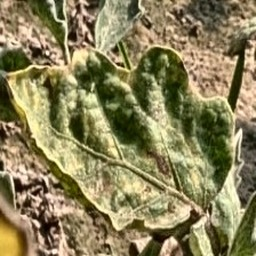
\includegraphics[width=8mm]{thumbs/s1v3.jpg}};
\node[stp, right=2.5mm of img] (s1) {\textbf{Structure view}\\blurred gray in a\\centred disc};
\node[stp, right=2.5mm of s1] (s2) {\textbf{Transform search}\\flips, quarter-turns,\\rotations, crops};
\node[stp, right=2.5mm of s2] (s3) {\textbf{Hubness correction}\\each image must\\single out the other};
\node[stp, right=2.5mm of s3] (s4) {\textbf{Label-calibrated null}\\other-class best\\match, Gumbel fit};
\node[stp, right=2.5mm of s4, draw=cblue, line width=0.85pt] (s5) {\textbf{Link if} $p{<}\alpha$\\group split or\\test filter};
\foreach \a/\b in {img/s1,s1/s2,s2/s3,s3/s4,s4/s5} \draw[arr] (\a) -- (\b);
\end{scope}
\end{tikzpicture}
\end{document}
